\chapter{Literature Review}
\label{ch:literature_review}
% \input{Sections/Ch3 Literature Review/Low SWaP Aerial Radar.tex}
% \input{Sections/Ch3 Literature Review/GPU radar processing performance.tex}
% \input{Sections/Ch3 Literature Review/Low SNR Monopulse feasability.tex}
% \input{Sections/Ch3 Literature Review/Programmable Vision Acceleration for Radar.tex}
% \input{Sections/Ch3 Literature Review/Summary.tex}

\section{Compact Airborne Radar for UAV DAA}
% Try to emphasise that there are not field trials that validate a full 
% target tracking pipeline under realistic encounter conditions
The work of Sysak et al.\ 
\cite{sysak2025_lightweight_compact_pulse_radar_uav_collision_avoidance}, 
Wang et al.\ \cite{Wang2016}, and Moses et al.\ \cite{6044363, Moses2015}
each tackle important subproblems in the design of a radar DAA system for 
small UAVs, but each leave important gaps unaddressed in the literature. 

Sysak et al.\ 
\cite{sysak2025_lightweight_compact_pulse_radar_uav_collision_avoidance} 
present a lightweight X-band monopulse radar for mid-air collision avoidance 
on medium UAV platforms, integrating a multi-channel forward-looking antenna 
with FPGA-based pulse compression on a single 60 gram PCB, with average power 
below 80 Watts. Field trials demonstrate reliable detection of large obstacles 
at 1--3 km (see Figure \ref{fig:sysak}), as well as detection of a 3.15 m 
wingspan UAV from 6.4 km. The work 
validates a simple online pipeline from range compression to \gls{tcpa} estimation,
but does not characterise the pipeline's latency or tracking performance, nor 
explain if the detections were make during sensing, or post-processed from recorded data. 

\begin{figure}
    \incfig[0.9]{sysak_radar}
    \caption{Sysak et al.'s experimental set up and results. The radar is 
    capable of detecting large targets at 1--3 km with high ranging accuracy. 
    We observe peaks in amplitude over range that correspond to target position.}
    \label{fig:sysak}
\end{figure}

Moses et al.\ \cite{6044363} in a 2013 publication introduces a 230 gram 
miniature radar mountable 
on a small quadcopter (see Figure \ref{fig:moses-quadcopter}), to demonstrate the feasibility of integrating radar
sensing onto very small platforms. Their evaluation emphasises target 
identification via 
micro-Doppler signatures rather than ranging or tracking, achieving a 100\% 
detection rate when 7 meters away from the target. When distance increased
and both the platform and target took to the air, accuracy dropped significantly.
This difference in performance between ground-based and airborne targets highlights
the importance of validating radar pipelines under realistic encounter conditions. 
While the work provides a dataflow diagram for the processing pipeline, it does not
characterise the latency of the stages not compare alternative algorithmic choices. 
Lastly, while the work discusses the difficultly of radar under SWaP-C constraints, 
the final weight, size, and power consumption of the radar system are not reported.

A follow up 2014 publication by the same group (Moses et al.\ \cite{Moses2015})  
presents an even smaller radar (see Figure \ref{fig:moses-2014}) with angle sensing 
capabilities and collision avoidance
algorithms, in attempt to further demonstrate more capabilities of miniature radar 
with respect to UAVs DAA systems. In this work, the radar is only evaluated indoors with large reflective 
targets. While the collision avoidance algorithms are compared thoroughly, no other
algorithm choices are evaluated and readiness for open air tests was not demonstrated.
For example, the authors note that a higher transmit power is needed. 

\begin{figure}[htbp]
    \centering
    \begin{minipage}{0.4\textwidth}
        \centering
        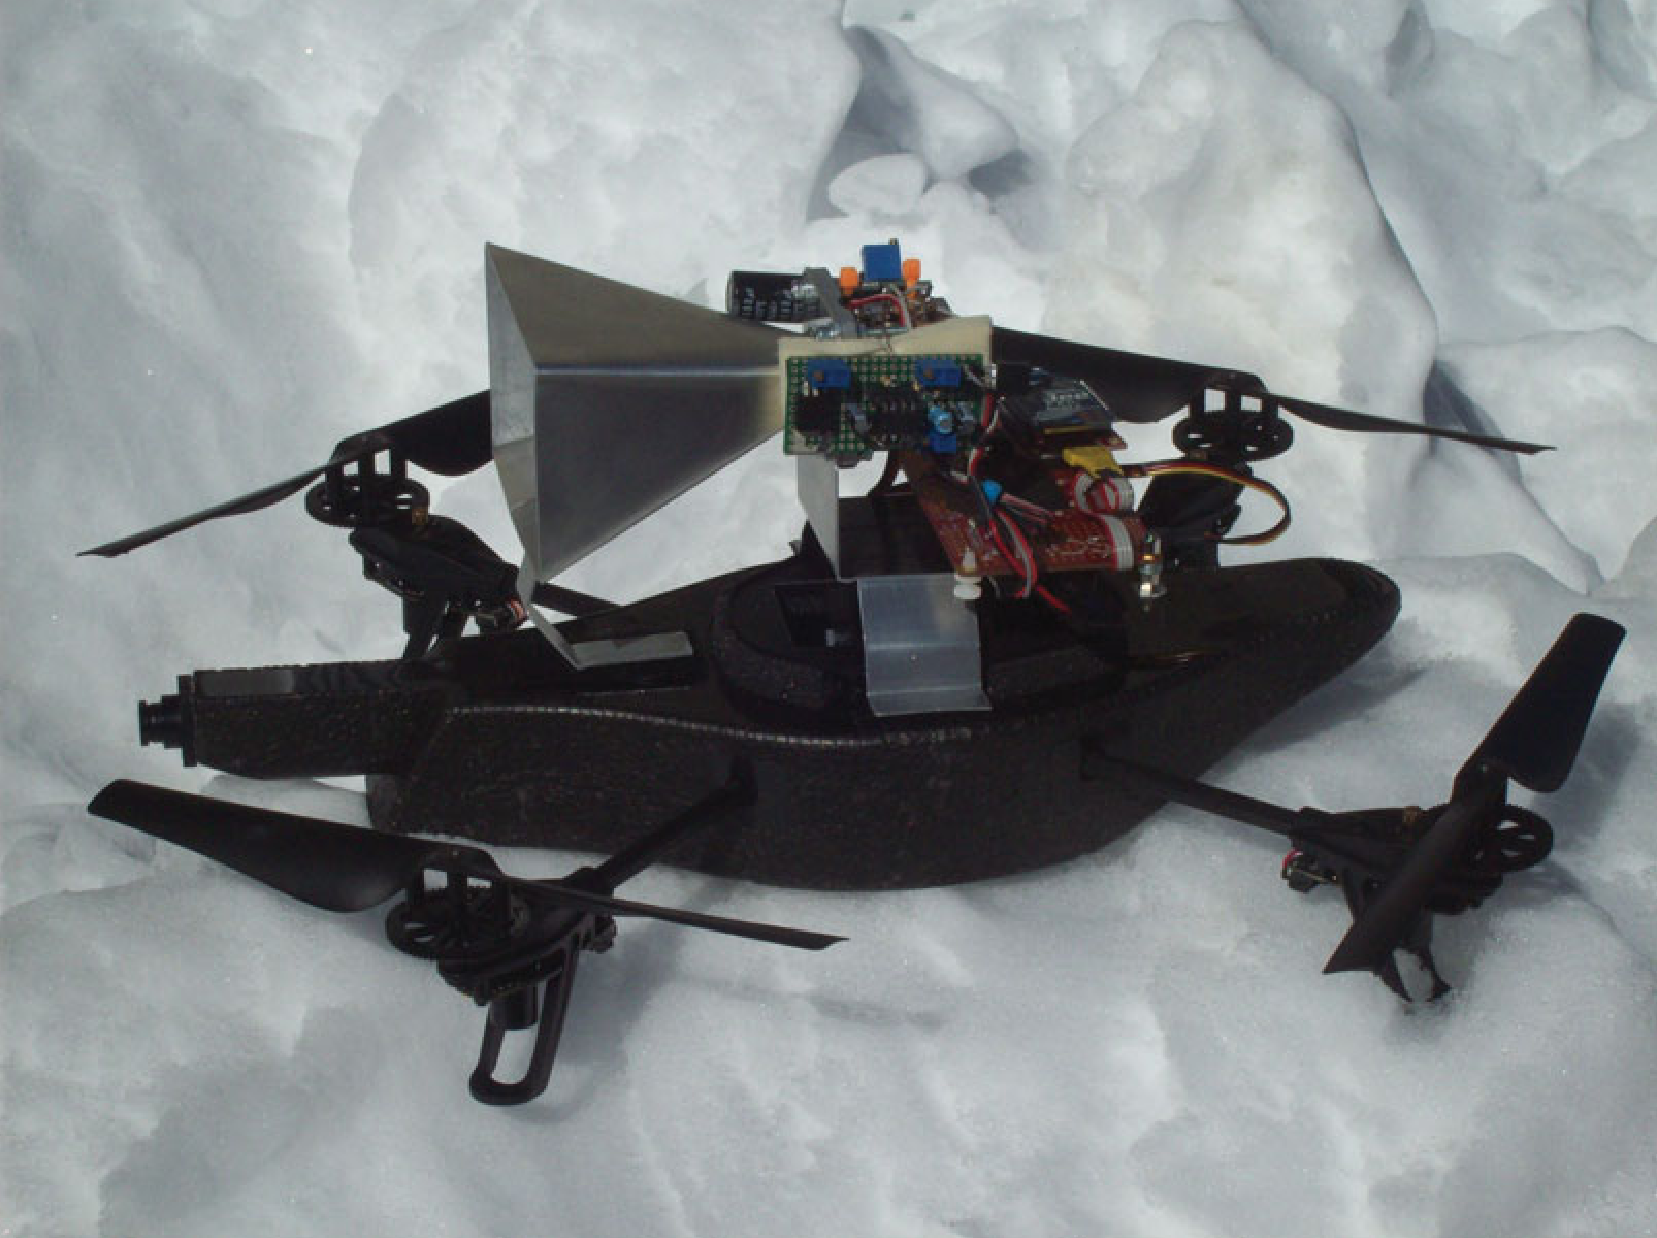
\includegraphics[width=\linewidth]{Moses 2013 quad copter.png}
        \caption{Moses et al.'s miniature radar mounted on a small quadcopter.}
        \label{fig:moses-quadcopter}
    \end{minipage}
    \begin{minipage}{0.4\textwidth}
        \centering
        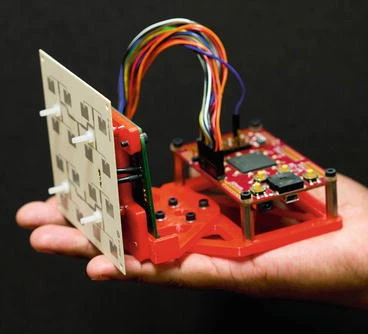
\includegraphics[width=\linewidth]{moses-2014.png}
        \caption{Second Generation of Moses et al.'s miniature radar, now
     with angle sensing capabilities.}
        \label{fig:moses-2014}
    \end{minipage}
\end{figure}

% Cool work that does ranging with big and small targets with light radar
% Pretty low-key research that just does some maths
% 
Wang et al.\ \cite{Wang2016} demonstrate a complete low-SWaP LFMCW system 
design for group 2/3 UAS (10-600 kg) group 2/3 UAS incorporating FFT-based 
detection, digital beamforming, and GPU-accelerated FFT for update rate 
improvement. The research highlights the feasibility of measuring the range
of targets 5+ km away through beamforming, but angle sensing capabilities were 
not explored. Additionally, design performance is validated in simulation only, 
and does not take into account compute and latency constraints. 
This thesis addresses these gaps by providing hardware-validated latency and 
throughput measurements for a comparable pipeline, and by substantiating the 
choice to use the GPU for certain operations with systematic benchmarks.

While research such as that of Mohammad Karimi et al. \cite{Mohammadkarimi2024} 
does support the feasibility of electronically scanning to measurement 
azimuth and elevation of targets, this work also does not characterise the
system in a realistic encounter scenario, only validating ranging and
angle estimation in simulation. While the work is rigorous in its mathematical
treatment of \gls{daa} requirements, empirical validation of the software
pipeline is needed to show that such a system can operate under the SWaP constraints
of a small \gls{uav}. 

Angle sensing, an important capability for UAV DAA, is not addressed
in Sysak et al.\ \cite{sysak2025_lightweight_compact_pulse_radar_uav_collision_avoidance},
Wang et al.\ \cite{Wang2016}, or Moses et al.\ \cite{6044363} \cite{Moses2015}, and is 
presented but not validated in Mohammad et al.\ \cite{Mohammadkarimi2024}. 

This thesis addresses these gaps by characterising the software pipeline by latency and
track quality, placing an emphasis on angle sensing, and by comparing the performance
of alternative algorithmic choices.  

This thesis addresses the gaps in Moses et al.'s work by evaluating the radar 
pipeline on real radar hardware data from open-air long-range scenarios, and 
by systematically comparing alternative algorithmic choices for each stage of 
the software pipeline, including FFT, integration, CFAR, monopulse angle sensing
and multi-target tracking under the SNR conditions characteristic of 
small-aperture UAV radars.

This thesis addresses the lack of empirically validated radar target tracking
pipelines by implementing a complete software pipeline and evaluating it and
comparing generated tracks to ground truth tracks. Additionally, attention will
be paid towards the ability for the pipeline to run in real time on board a small
\gls{uav}. 

\section{GPU-based Radar Processing Under SWaP Constraints}
The work of Shi et al.\ \cite{6712628}, Newmeyer et al.\ \cite{7577322}, 
Zhao et al.\ \cite{rs15225421}, and Zaknoun 
\cite{zaknoun2024_realtime_gpu_accelerated_radar_processing} 
each explore the computational challenges of small airborne radar systems
across different contexts. Still important gaps remain unaddressed across 
all literature.

Shi et al.\ \cite{6712628} describe a small \gls{fmcw} phased array built from 
off-the-shelf development boards, validating that continuous real-time 2D FFTs 
are achievable on a 100 MHz FPGA. However, processing was split between an 
onboard FPGA and offboard post-processing, and signal coherence problems 
prevented real-world validation. This thesis addresses this gap by implementing 
a fully onboard, online pipeline and validating it against real target returns.

Newmeyer et al.\ \cite{7577322} demonstrated a 120 gram, 8 Watt \gls{fmcw} phased 
array pipeline on a Zynq ARM CPU, closely monitoring power, latency 
distributions, and hardware resources. This work clearly establishes that 
radar DAA can operate under strict SWaP constraints. However, only one 
hardware configuration and one algorithm sequence are evaluated. This thesis 
addresses this gap by systematically comparing alternative algorithmic 
pathways and evaluating how pipeline bottlenecks change across embedded 
compute configurations, including GPU-based architectures.

Zhao et al.\ \cite{rs15225421} implement CUDA acceleration for a passive 
bistatic radar pipeline, reporting up to a 113.13$\times$ speedup over a CPU 
baseline across three algorithm stages. However, the study covers only clutter 
suppression, range--Doppler processing, and CA-CFAR detection, omitting angle 
estimation, coordinate transforms, and Kalman filtering, and does not discuss 
memory reallocation or thread synchronisation costs. This thesis addresses 
these gaps by benchmarking a more comprehensive algorithm selection and 
profiling host--device transfer and synchronisation overhead explicitly.

Zaknoun \cite{zaknoun2024_realtime_gpu_accelerated_radar_processing} provides 
a comprehensive treatment of GPU radar software architecture for real-time 
processing. However, this work is not situated in a UAV DAA context and does 
not evaluate performance under UAV SWaP constraints. This thesis adapts these 
architectural insights to the UAV DAA problem, evaluating how conclusions 
change under constrained power and memory budgets.

\section{Sensitivity and Detection in Low-SNR Regimes}

A key consequence of SWaP-constrained hardware is reduced aperture, which 
simultaneously lowers SNR and degrades angular resolution, increasing the 
likelihood that multiple targets occupy the same resolution cell.

An et al.\ 
\cite{an2024_time_varying_angle_estimation_unresolved_extended_targets_monopulse} 
propose an efficient method for resolving two unresolved targets within a 
single monopulse cell. However, evaluation is limited to simulated white-noise 
conditions, the method is not integrated into an end-to-end range--Doppler 
pipeline, and explicit failure modes exist for same-angle targets and 
cells containing three or more targets. This thesis addresses these gaps by 
testing the algorithm under non-white noise conditions and within a complete 
tracking pipeline, measuring the effect on track quality.

Aubry et al.\ 
\cite{aubry2020_single_pulse_simultaneous_detection_angle_estimation_multichannel} 
demonstrate that detection and angle estimation can be treated jointly in a 
multichannel array, increasing sensitivity to targets not visible in any single 
channel and avoiding the brittleness of early thresholding under low SNR. 
However, validation is limited to single simulated targets in Gaussian 
interference. This thesis addresses this gap by applying the algorithm to 
multiple targets under non-Gaussian noise regimes and measuring both 
sensitivity and track-quality impacts alongside compute cost.

The noise and clutter regime experienced by a miniature airborne radar has not been empirically
characterised in the literature. Ezuma et al.\ \cite{ezuma2019microuav} demonstrate that
Gaussian and Rayleigh clutter assumptions — the basis of CA-CFAR — already fail for
ground-based mmWave radar detecting UAVs, finding that a Weibull distribution provides a
significantly better fit to the measured clutter statistics, and explicitly noting that prior
UAV detection work had neglected this. The airborne case, where the radar sensor is itself
mounted on a vibrating UAV platform subject to altitude variation, aspect angle changes, and
platform-induced interference, introduces further departures from the homogeneous Gaussian
noise model that underpins standard windowing and CFAR algorithm selection. No published work
has measured or modelled these statistics for a miniature airborne FMCW radar in real flight
conditions. As a result, the algorithm choices made in existing pipeline designs, (window
function selection, CFAR variant, and training cell configuration) lack empirical
justification for this operating regime.

\section{Summary and Research Gap}
Across the UAV DAA radar literature three gaps emerge. First, existing 
hardware demonstrations validate detection against large, high radar 
cross-section targets only; no work characterises sensitivity to small 
moving airborne targets under realistic encounter conditions. Second, 
processing feasibility on constrained embedded hardware has been demonstrated 
on FPGAs and ARM CPUs, but no work benchmarks a GPU-based pipeline in a UAV 
DAA context with comprehensive algorithm coverage and architectural profiling. 
Third, the noise and clutter regime of miniature airborne FMCW radar has not been empirically
characterised. Existing work shows that Gaussian clutter assumptions fail even for ground-based
mmWave radar, yet no study has measured these statistics for an airborne sensor. As a result,
the window function, CFAR variant, and training cell choices made in existing pipeline designs
lack empirical justification for this operating regime, and angle sensing algorithms have only
been validated under idealised white Gaussian noise with single simulated targets.

This thesis addresses all three gaps by characterising detection and tracking
sensitivity against small moving airborne targets, by benchmarking a
comprehensive selection of radar processing and tracking algorithms on embedded
GPU hardware with explicit profiling of host--device transfer and
synchronisation overhead, and by collecting real flight data to characterise the
noise regime and evaluate monopulse angle sensing algorithms within a complete
multi-target tracking pipeline under realistic conditions.